\vspace{-1mm}
\section{Agent Workflow Memory}
\label{sec:3:method}
% \vspace{-2mm}

In this section, we first describe the web navigation task (\S\ref{sec:3.1:problem-statement}), then introduce the workflow representation (\S\ref{sec:3.2:workflow-repr}), and describe the mechanism of \awm as well as various instantiations (\S\ref{sec:3.3:atm}).

%%%%%%%%%%%%%%%%%%%%%%%%%%%%%%%%%%%%%%%%%%%%%%
% \vspace{-1mm}
\subsection{Problem Statement}
\label{sec:3.1:problem-statement}

For the purpose of this paper, we consider agents with a language model backbone $L$ and text-based memory $M$, where the base memory contains documentation of built-in actions such as \texttt{CLICK} and \texttt{TYPE}.\footnote{Memory is usually implemented as a system prompt or auxiliary information in the main prompt context.} To solve a task specified by a natural language (NL) instruction $q$, the agent acts in an environment defined by a transition function $T$. 
For each time step $t_i$, the environment state $s_i$ gives observation $o_i$, which is then passed into the model to generate action $a_i$ via $L(q, M, o_i) \rightarrow a_i$. The action is executed in the environment and changes the state as $T(s_i, a_i) \rightarrow s_{i+1}$. This observe-act loop iterates until the model predicts the stop action $a_i = $\verb|STOP|, or reaches a task termination condition, \eg, a maximum pre-determined number of steps.


Each completed task forms an experience $e$, which comprises an NL instruction $q$ and a trajectory of steps attempting to solve the task, where each step $p$ contains the agent observation $o$ obtained from the current state, and action taken by the agent $a$, formulated as $p = (o, a)$. 
Our goal is to induce useful workflows $\mathcal{W}=\{w\}$ from the set of experiences $\mathcal{E}=\{e\}$ constructed from past or collected examples, using an induction module $I$ via $I(\mathcal{E}) \rightarrow \mathcal{W}$. We add induced workflows into the agent memory $M$ as guidance for subsequent task-solving. 

Next, we introduce the workflow representation design, workflow induction method, and agent memory update with workflows in varied setups.



%%%%%%%%%%%%%%%%%%%%%%%%%%%%%%%%%%%%
% \vspace{-2mm}
\subsection{Workflow Representation}
\label{sec:3.2:workflow-repr}
\vspace{-1mm}

Similar to an experience, a workflow comprises two components: first, a textual description of the workflow $d$; and second, a series of steps to finish the workflow $(p_1, p_2, \cdots)$, as shown in \autoref{fig:awm-pipeline}. 

\begin{wrapfigure}[16]{r}{0.6\textwidth}
\vspace{-6mm}
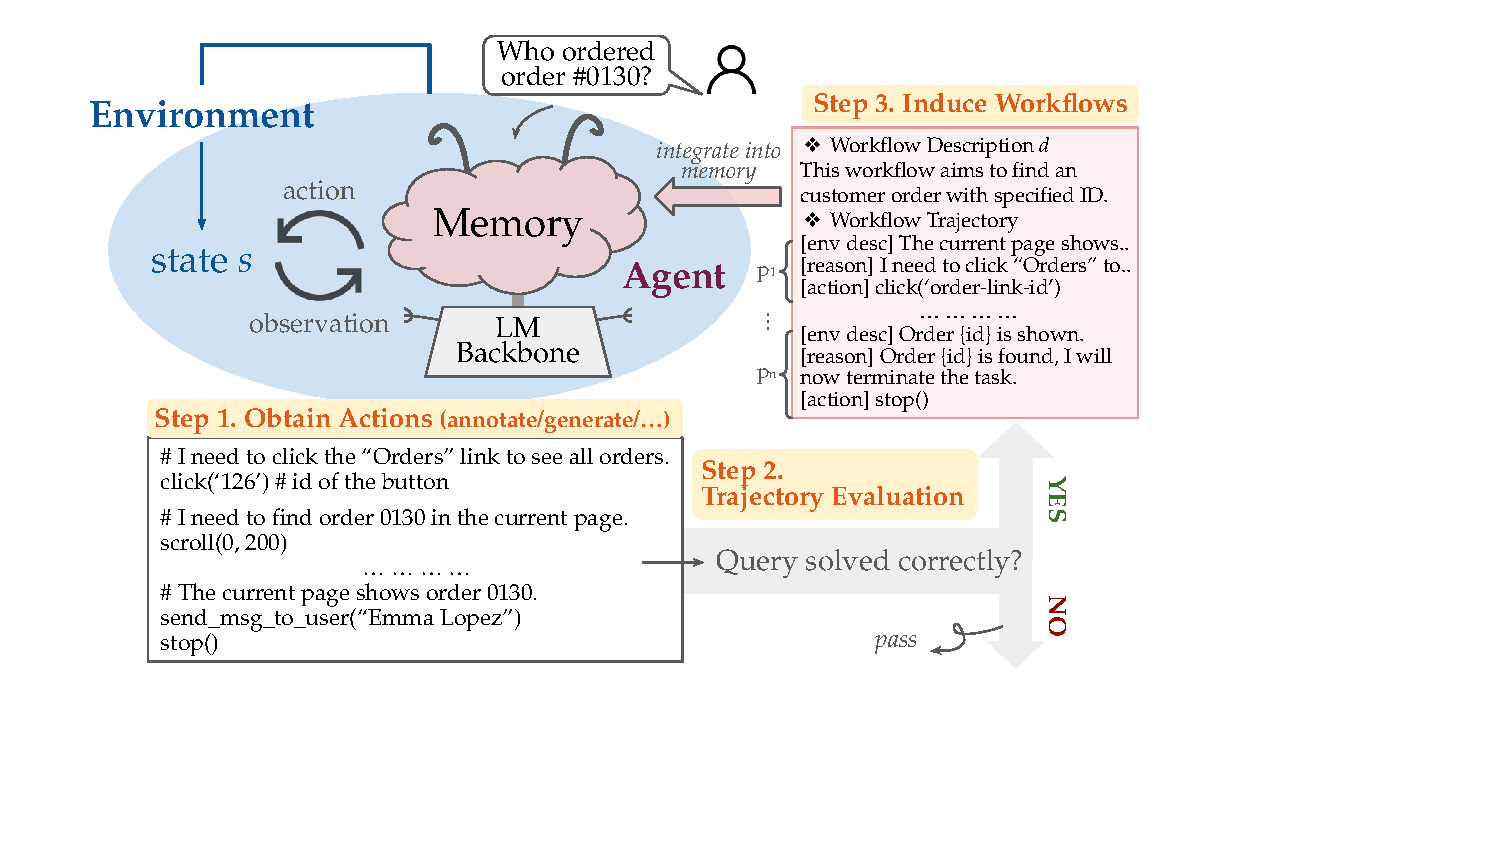
\includegraphics[width=0.6\textwidth]{./figures/awm-pipeline.pdf}
\vspace{-7mm}
\caption{Illustration of our \awm pipeline: an agent takes actions to solve given queries, induces workflows from successful ones, and integrates them into memory.}
\label{fig:awm-pipeline}
\vspace{-3mm}
\end{wrapfigure}

\noindent \textbf{Workflow Description} \quad
To present workflows in a format where agents can learn from them properly, it is important to describe the high-level goal of the series of actions. Therefore, we associate each workflow with an NL task description $d$, essentially a summary of the workflow's function, by heuristically extracting from experience instructions or summarizing with an LM (see \S\ref{sec:3.3:atm}).


\noindent \textbf{Workflow Trajectory} \quad
The workflow trajectory contains a series of steps $(p_1, p_2, \cdots)$ to finish the process described in $d$. Each $p$ consists of three parts, demonstrated in $p_n$ in \autoref{fig:awm-pipeline}, Step 3. (1) A description of the current environment state in NL, such as ``Order \{id\} is shown''; (2) The reasoning process elaborated by the agent to decide which action to generate based on observations, such as ``Order \{id\} is found, I will now terminate the task.''; and (3) an action represented as an executable program over the environment, \ie, \texttt{stop()} that realizes termination.


%%%%%%%%%%%%%%%%%%%%%%%%%%%%%%%%%%%%%%%%%%%%
% \vspace{-1mm}
\subsection{Inducing and Using Workflows}
\label{sec:3.3:atm}
At the core of AWM is an induction module $I$ that induces a set of workflows $\mathcal{W}$ from one or more past agent experiences $\mathcal{E} = \{e_i\}_{i=1}^{m}$. Each experience $e = (q, P^e)$ contains an NL task instruction $q$ and an action trajectory that consists of a sequence of steps (observation and action) $P^e = (p^e_1, ..., p^e_n)$ that were taken to solve $q$. The workflow induction module operates by taking in $\mathcal{E}$ and producing a set of workflows, as $I(\mathcal{E}) \rightarrow \mathcal{W} = \{w\} = \{(d_j, P_j^d)\}$.

\vspace{-2mm}
\paragraph{LM-based Workflow Induction}
To produce workflows that more accurately capture reusable trajectories across tasks, we propose an LM-based module $I$ that prompts the agent to extract common sub-routines from one or more input experiences. 

Different from task instructions that specify concrete, less-repetitive tasks, \eg, ``Buy dry cat food on Amazon and deliver to my address'', we deliberately prompt models to induce workflows at finer granularities, \ie, a sub-task ``search for a product on Amazon'' that frequently re-appears as part of multiple similar instructions.
Meanwhile, instead of giving example-specific values (\eg, ``dry cat food''), we enhance workflow generality by abstracting out example-specific contexts, \ie, replacing ``dry cat food'' with a more general name ``\{product-name\}'' by specifying this in the workflow induction prompts. 
These workflows are segmented (based on double-line breaks in the model output) and stored separately in the workflow memory.
See \S\ref{app:lm-induction-details} for the model prompts, example workflows, and an examination of quality.\footnote{We also explore a rule-based workflow induction method. See \S\ref{app:rule-induction} for more detailed experiments.}


\begin{wrapfigure}[8]{r}{0.43\textwidth}
\vspace{-9mm}
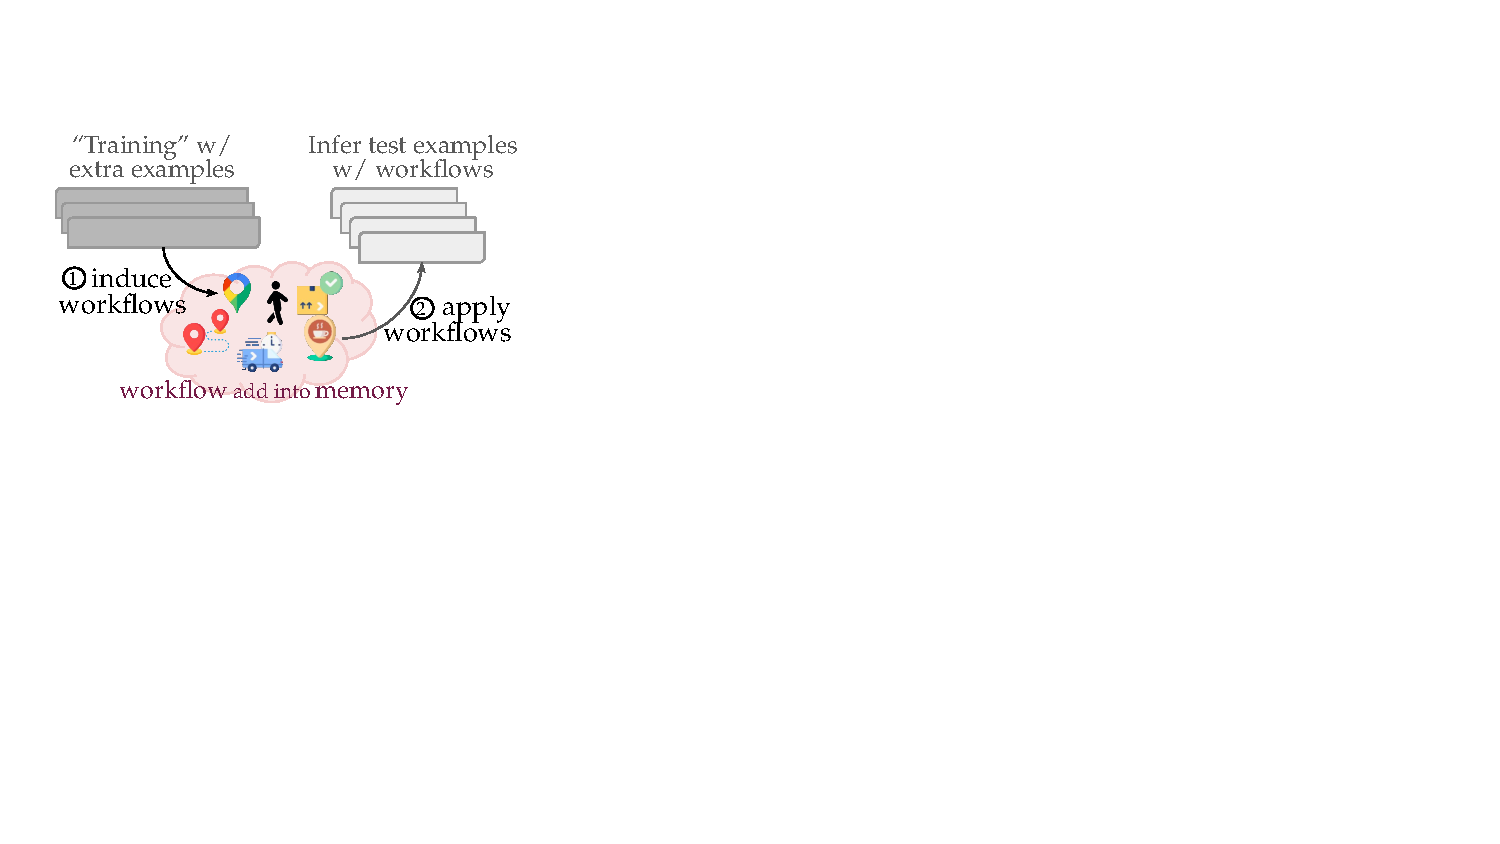
\includegraphics[width=0.42\textwidth]{./figures/offline-process.pdf}
\vspace{-4mm}
\caption{Illustration of \textsc{AWM}$_{\it offline}$.}
\label{fig:offline-process}
% \vspace{-2mm}
\end{wrapfigure}
% using
After the workflows $\mathcal{W}$ are induced, they are then integrated into the agent as auxiliary memory, $M + \mathcal{W} \rightarrow M_w$, where $M$ stands for the original agent memory, and $M_w$ stands for the agent memory augmented with induced workflows.
When solving a given instruction $q$, the agent now produces a series of actions by $L(q, M_w, o) = L(q, M + W, o) \rightarrow a$.
In the following, we introduce \awm in use in two scenarios:

\vspace{-1mm}
\paragraph{Offline Scenario}
% \label{sec:3.3.1:offline}
% \vspace{-1mm}
\awm can operate in an \emph{offline} scenario when additional canonical experiences are available, such as data annotated by humans or synthesized by models. In this case, we perform workflow induction and utilization in two standalone processes. 
As seen in \autoref{fig:offline-process}, \awm first takes in all training examples from a website by concatenating them into a single prompt, and feeds them to the LM to create a set of workflows at `training' time; $I(\mathcal{E}_{\it train}) \rightarrow \mathcal{W}_{\it offline}$. 
Second, \awm incorporates all induced workflows into the agent memory at inference time to solve test instructions $L(q, M + \mathcal{W}_{\it offline}, o_i^{\it test}) \rightarrow a_i^{\it test}$. Since the workflows are fully induced before test-time inference, the agent uses the same workflow memory $\mathcal{W}_{\it offline}$ to solve each test.

\vspace{-1mm}
\paragraph{Online Scenario}
% \label{sec:3.3.2:online}
% \vspace{-1mm}
Extra canonical experiences are not always available or easy to collect, especially those that cover the same domains and tasks as the test instructions. \awm also works in an online, supervision-free setting, where only test queries are needed.
Agents with \textsc{AWM}$_{\it online}$ process test queries in a streaming fashion, where the agents conduct the loop of induce, integrate, and utilize workflows after running inference for each test task. 

\begin{wrapfigure}[10]{r}{0.45\textwidth}
\vspace{-7mm}
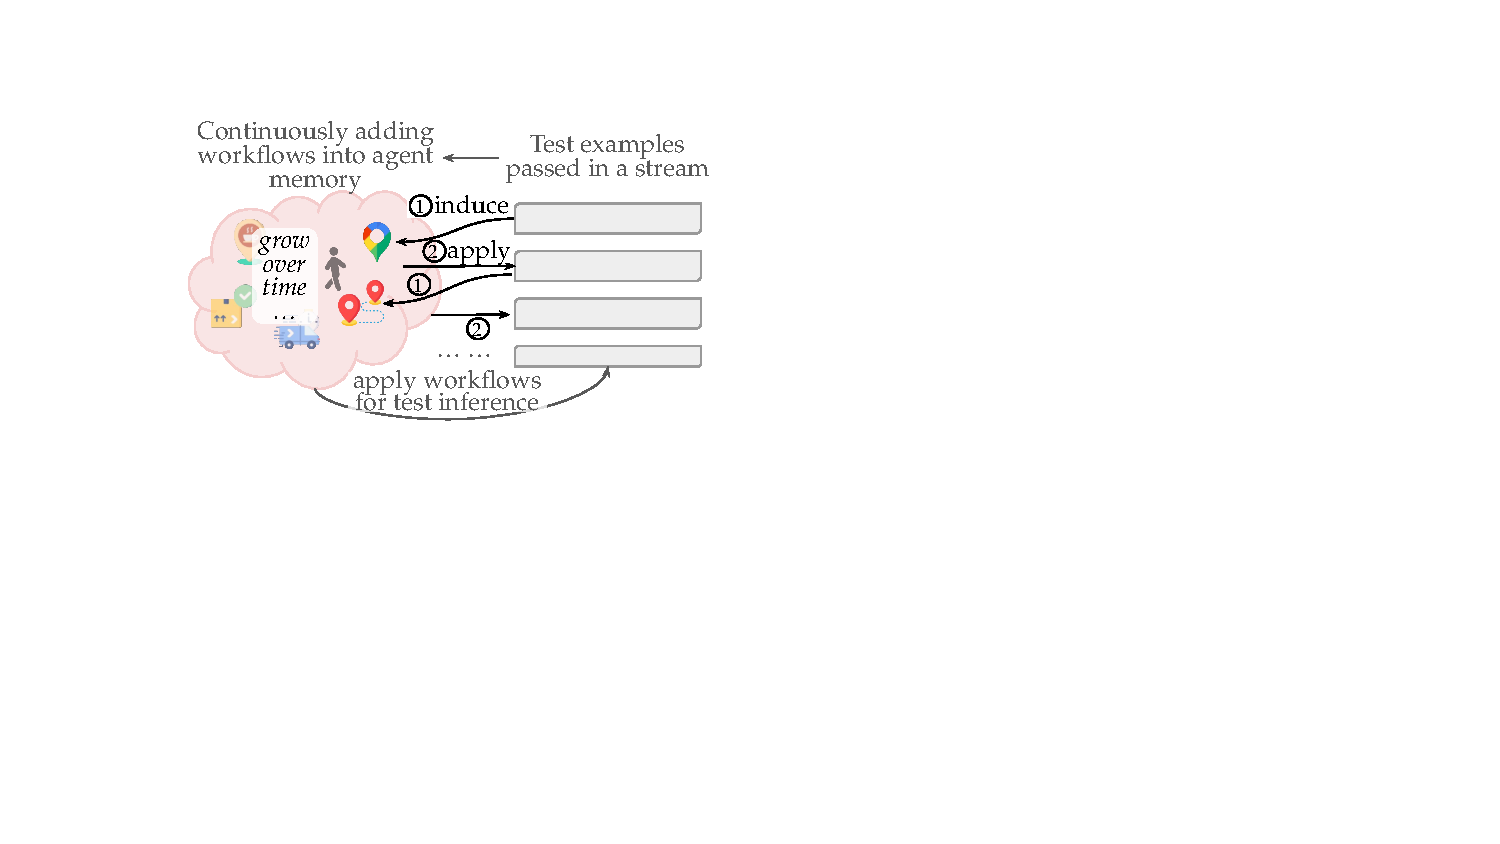
\includegraphics[width=0.44\textwidth]{./figures/online-process.pdf}
\vspace{-3mm}
\caption{Illustrations of \textsc{AWM}$_{\it online}$.}
\label{fig:online-process}
% \vspace{2mm}
\end{wrapfigure}

Concretely, the agent starts with the default memory $M$; 
given the $t$-th test instruction $q_t$ passed into the agent, the agent attempts to solve the task by generating an action trajectory $(p^t_1, p^t_2, \cdots)$, which collectively forms an experience $e_t = (q^t, \{p^t\})$. We adopt the LM-based evaluation model of  \citet{pan2024autonomous} to output a binary label, $L_{\it eval}(e^t) \in \{0, 1\}$, that judges if $e^t$ successfully solves $q^t$ by prompting a neural model. If $e^t$ is predicted as success, \ie, $1$, we then transform it into workflow(s) $I(e^t) \rightarrow \{w^t\}$ and add $\{w^t\}$ into the agent memory $M^t + \{w^t\} \rightarrow M^{t+1}$, which serves as the agent memory to process the $t+1$-th instruction.
As depicted in \autoref{fig:online-process}, we continue this memory-updating process by iteratively predicting actions for and inducing workflows from streamed test instructions, until all tests are processed. We evaluate the success rate of the predicted action trajectories $\{p^t\}$ for all tests and report the average score.
